\section{Prospettive sulla programmazione parallela}
Uno degli aspetti più importante è analizzare il problema e capire se può essere parallelizzato. La parallelizzazione del codice parta a dei miglioramenti delle performance solo se il workload (peso computazionale) è non indifferente.


Partiamo con un po' di definizioni:
\begin{itemize}
    \item Task: arbitrario pezzo di lavoro/sequenza di codice in una computazione parallela. Viene eseguito sequenzialmente, la concorrenza si ha solo tra le task;
    una task è una sequenza di istruzioni che andiamo a identificare, è una parte del programma.
    \item Processo/thread: entità astratta che performa le task assegnate ai progetti. I processi comunicano e si sincronizzano per eseguire le lo task.
    \item Processore: motore fisico sul quale si eseguono i processi. Più thread possono essere eseguiti sullo stesso processore, un thread non può essere eseguita su più processori.
\end{itemize}

\subsection{Step per creare un programma parallelo}
Possiamo identificare 4 passi nella creazione di un programma parallelo:
\begin{enumerate}
    \item Decomposizione della computazione in task -> parto dall'algoritmo risolutivo e identifico tutte le task che lo compongono (divido il problema in sottoproblemi);
    \item Assegnamento delle task ai processi (mappiamo le task identificate nelle thread disponibili); 
    \item Orchestrazione degli accessi ai dati, della comunicazione e della sincronizzazione -> si capisce come raggruppare i processi in unità da eseguire in parallelo;
    \item Mapping dei processi ai processori. Ovviamente, un processo non può essere assegnato a più unità di calcolo.
\end{enumerate}

Le fasi di \textbf{decomposizione} e \textbf{assegnamento} compongono la fase di partizionamento del problema (partiamo da un problema grosso e lo dividiamo su processi computazionale). Qui in pratica è dove identifichiamo il livello di parallelismo.

\subsubsection{Comprensione del problema/programma}
Il primo reale step da eseguire resta però il capire il problema e/o il programma. Se stiamo partendo da un programma sequenziale già scritto, dobbiamo per forza capire come funziona per poterlo parallelizzare, mentre nel caso del problema dobbiamo capire se questo è anche parallelizzabile. 
In generale quello che dobbiamo fare è:
\begin{enumerate}
    \item Identificare gli hotspot del programma: rappresentano le parti più "pesanti" del codice e sono solitamente identificati dopo aver fatto profiling\footnote{I tool di profiling eseguono il codice e, assieme al suo risultato, ritornano anche un report che può contenere: il numero di invocazioni a funzione per ogni funzione del codice, il tempo impiegato da ogni esecuzione di ogni funzione, quali parti del codice sono più usate, ...} e analisi delle performance (tramite appositi tool). Gli hotspot sono generalmente le sezioni in cui si concentra la parallelizzazione.
    \item Identificare i bottleneck del programma: rappresentano i punti del codice che sono più lente ad eseguire (come ad esempio le sezioni dedicate all'I/O). Una possibile strada che si può seguire per i bottleneck consiste nel trasferire la loro esecuzione sulla GPU, in modo da non dover rallentare la CPU. Possiamo quindi vedere due livelli di parallelismo: il primo dato dalla GPU che parallelizza la funzione, mentre il secondo dato dalla concorrenza di esecuzione di CPU e GPU.
    \item Identificare gli inibitori al parallelismo: analizzare il problema significa anche identificare gli inibitori del parallelismo, che sono quei fattori che impediscono di parallelizzare il codice. Generalmente, un inibitori dal parallelismo è la dipendenza delle task, dove il risultato di quella successiva dipende dal risultato di quella precedente.
\end{enumerate}

\underline{Esempio di problema parallelizzabile}: Calcolare l'energia potenziale per ciascuna delle diverse migliaia indipendenti Conformazioni di una molecola. Al termine, trova la conformazione energetica minima. Ogni conformazione molecolare è indipendentemente determinabile e il calcolo della conformazione energetica minima è parallelizzabile.
\\

\underline{Esempio di problema non-parallelizzabile}: Calcolare la serie di Fibonacci. Questo problema non è parallelizzabile in quanto il calcolo attuale dipende dai calcoli precedenti (il termine $k+2$ è dato dalla somma dei termini $k+1$ e $k$). 
\\



\subsubsection{Decomposizione}
Nella scomposizione andiamo ad identificare task sufficiente affinché ce ne sia abbastanza da poter tenere le thread, e i corrispondenti processori, sempre occupati. Questo significa che se abbiamo una macchina con 100 processori, che possono andare tutti in parallelo, dobbiamo avere un pool di task sufficientemente grande da poter tenere occupati tutti i processori anche nel momento in cui una delle task si blocca. Infatti capiterà che una task arrivi al punto in cui necessità di dati da un'altra task o di eseguire operazioni di I/O, restando quindi bloccata e lasciando inutilizzato il processore. Quello che vogliamo evitare è appunto il suo utilizzo, che possiamo evitare se disponiamo di un'altra task pronta ad essere eseguita appena un processore si libera. Dei core/processori lasciati in stallo (inutilizzati) ci ritroviamo con uno spreco di risorse.
Per farla semplice, ci serve un numero di task sufficiente a permetterci di rimpiazzare immediatamente quelle "bloccate" per evitare l'inutilizzo dei processori.

Esistono due modi per scomporre in task:
\begin{itemize}
    \item Scomposizione di dominio: prevede di scomporre i dati del problema, facendo lavorare poi ogni task su una porzione dei dati. Esistono vari modi di partizionare i dati, la soluzione migliore generalmente dipende dal modo in cui sono memorizzati i dati sul pc.

    I problemi, che siano monodimensionale che bidimensionali, possono essere scomposti, ad esempio, in blocchi o cicli (figure \ref{fig:domain-decomposition}). Un fattore importante da tenere presente è il bilanciamento del carico. se siamo sicuri che il tempo impiegato dalla prima thread sul blocco A corrisponde a quello impiegato dalla seconda thread sul blocco B e così via per il resto dei blocchi, allora abbiamo un carico bilanciato. Questo di solito è il caso per problemi lineari. Quando però abbiamo problemi più complessi, il carico di lavoro di una thread diventa imprevedibile. In questo caso potrebbe essere più ottimale aumentare i blocchi facendo in modo che il primo processore che si libera vada a prendere la successiva thread in attesa.
    \begin{figure}[th]
    	\centering
    	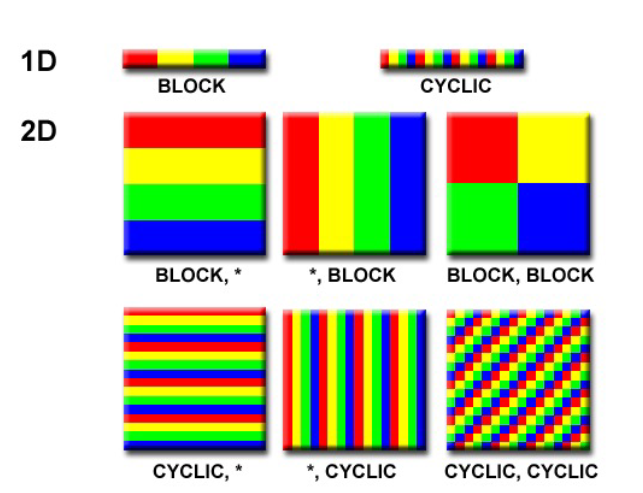
\includegraphics[width=0.7\linewidth]{img/domain-decomposition.png}
    	\caption{Esempio di decomposizione del dominio.}
    	\label{fig:domain-decomposition}
    \end{figure}

    \item Scomposizione funzionale: ci si concentra sull'elaborazione che deve essere fatta piuttosto che sui dati manipolati dalla computazione. Il problema è quindi scomposto rispetto al lavoro che deve essere fatto. Ogni task esegue parte del lavoro totale.
\end{itemize}

La scomposizione è compito del programmatore, che può essere supportato da tool automatici (campo di ricerca).

\underline{Esempio di parallelizzazione}
\\

Data un'immagine $NxN$ vogliamo:
\begin{itemize}
    \item Raddoppiare la luminosità di ogni pixel;
    \item Calcolare la media di tutti i pixel.
\end{itemize}

Una risoluzione sequenziale di questo problema costa un tempo totale di $2N^2$, con ogni step che ne costa $N^2$ (figure \ref{fig:esecuzione-sequenziale}). 
\begin{figure}[th]
	\centering
	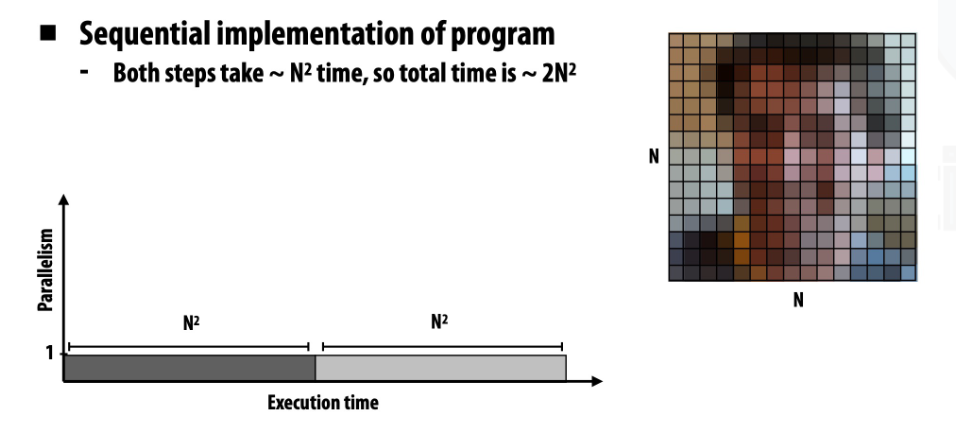
\includegraphics[width=0.7\linewidth]{img/esecuzione-sequenziale.png}
	\caption{Esecuzione sequenziale.}
	\label{fig:esecuzione-sequenziale}
\end{figure}

Una possibile strategia di parallelizzazione potrebbe consiste nell'eseguire in parallelo lo step 1, portando il tempo necessario a completare questa fase a $N^2/P$ (figure \ref{fig:esecuzione-parallela-1}), dove $P$ rappresenta il numero di processori disponibili. Lo speedup ottenuto sarebbe:
\begin{align*}
    speedup &\le \frac{2n^2}{\frac{n^2}{p} + n^2}\\
    &\le 2
\end{align*}

\begin{figure}[th]
	\centering
	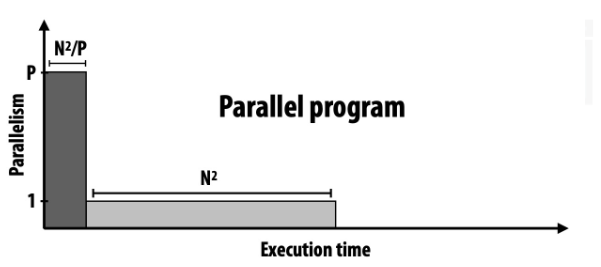
\includegraphics[width=0.7\linewidth]{img/esecuzione-parallela-1.png}
	\caption{Primo tentativo di parallelismo.}
	\label{fig:esecuzione-parallela-1}
\end{figure}

Una strategia più efficiente consiste nel parallelizzare parzialmente anche il secondo step, computando le somme parziali in parallelo (figure \ref{fig:esecuzione-parallela-2}). I tempi diventano:
\begin{align*}
    \text{Tempo step 1 } &= \frac{N^2}{P}\\
    \text{Tempo step 2 } &= \frac{N^2}{P} + P\\
\end{align*}

con speedup:
\begin{align*}
    speedup \le \frac{2n^2}{\frac{n^2}{p} + p}\\
\end{align*}

\begin{figure}[th]
	\centering
	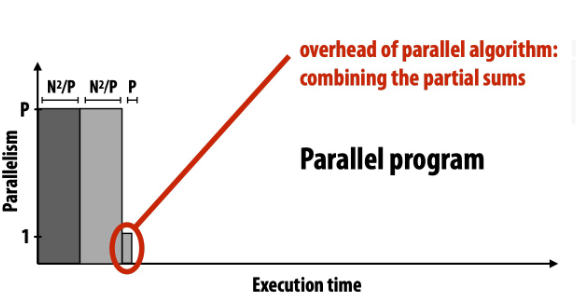
\includegraphics[width=0.7\linewidth]{img/esecuzione-parallela-2.png}
	\caption{Secondo tentativo di parallelismo.}
	\label{fig:esecuzione-parallela-2}
\end{figure}

\subsubsection{Assegnamento}
In questa fase andiamo a specificare il meccanismo con cui dividere le task tra i processi. Per semplicità, possiamo vedere le task come "cose da fare", mentre i processi/thread come i "lavoratori". Abbiamo fatto la scomposizione, sappiamo quanti e quali sono le thread, cerchiamo ora di fare un assegnamento che ci garantisca un certo livello di carico. 
Un approccio strutturato solitamente funziona bene, possiamo seguire euristiche ben conosciute o anche ispezionare attentamente il codice.


Il \textbf{load balancing} (bilanciamento del carico di lavoro) fa riferimento alla pratica di distribuzione delle task tra le thread affinchè tutte le thread siano occupate tutto il tempo. Possiamo anche definirlo come la riduzione al minimo dei tempi di inattività del processo. Questo passo è molto significativo per le perfromance. Ad esempio, se tutti i processi fossero soggetti ad un punto che funge da barriera di sincronizzazione, le performance globali verrebbero determinate dalla task più lenta.
\begin{figure}[th]
	\centering
	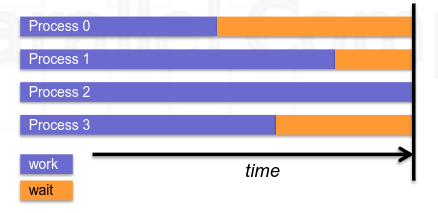
\includegraphics[width=0.7\linewidth]{img/barrier-sync.png}
	\caption{Esempi di punto di sincronizzazione.}
	\label{fig:barrier-sync}
\end{figure}

Possiamo ottenere il load balancing in più modi:
\begin{enumerate}
    \item Dividendo equamente le task tra i processi disponibili:
    \begin{itemize}
        \item In caso di operazioni su array/matrici, dove ogni processo esegue operazioni simili, il dataset viene distribuito in modo uniforme tra i processi;
        \item Per le iterazioni di un ciclo dove il lavoro svolto da ogni loop è similare, le iterazioni vengono distribuite uniformemente tra i processi;
        \item Se si utilizza un mix eterogeneo di macchine con performance variabili, è consigliato utilizzare dei tool di analisi delle performance per individuare carichi sbilanciati e aggiustare di conseguenza.
    \end{itemize}
    \item Usando un assegnamento dinamico del lavoro: alcune classi generano un carico di lavoro sbilanciato anche se i dati sono distribuiti egualmente tra il processi, come:
    \begin{itemize}
        \item Array sparsi;
        \item Adaptive grid methods, dove alcuni processi potrebbero dover perfezionare la propria mesh, mentre altri no;
        \item N-body simulations, dove alcune particelle potrebbero migrare verso/dal dominio del proprio processo di origine verso quello di un altro processo, oppure dove alcune particelle richiedono più lavoro rispetto ad altre.
    \end{itemize}
    Quando l'ammontare di lavoro che ogni thread performerà è variabile (non intenzionalmente ovviamente), è utile usare un approccio \textbf{scheduler – task pool}. In questo modo, appena un processo finisce, si mette in coda per ottenere un nuovo pezzo di lavoro.
    Inoltre, potrebbe diventare necessario disegnare un algoritmo che rileva e gestire sbilanciamento mentre questi si verificano dinamicamente nel codice.
\end{enumerate}

La \textbf{granularità} rappresenta una misura qualitativa del rapporto tra computazione e comunicazione. Generalmente i periodi di computazione sono separati da quelli di comunicazione da eventi di sincronizzazione. Relativamente al parallelismo, la granularità si divide in:
\begin{itemize}
    \item Fine grain parallelism (parallelismo a grana fine): si effettuano relativamente piccole quantità di lavoro computazionale tra gli eventi di comunicazione. Abbiamo quindi un basso rateo tra computazione e comunicazione. Facilita il load balancing; implica un elevato overhead di comunicazione e meno opportunità per il miglioramento delle performance. Se la granularità è troppo fine è possibile che l'overhead richiesto per comunicazione ee sincronizzazione tra le task richieda più tempo della computazione vera e propria.





    \item Coarse grain parallelism (parallelismo a grana grossa): si effettuano relativamente grandi quantità di lavoro computazionale tra gli eventi di comunicazione/sincronizzazione. Abbiamo quindi un alto rateo tra computazione e comunicazione. Implica più opportunità per un incremento delle performance, ma rende più difficile bilanciare il carico di lavoro efficientemente
\end{itemize}










